%-------------------------------------------------------------------------
% Design Project Input/Output Module Description
%-------------------------------------------------------------------------

\clearpage
\section{Light Input Module}
\label{sec-input-light}

This input module enables your IoT device to sense how much light is
reaching the device. The module uses a small photo-resistor which is
similar in spirit to the potentiometer you experimented with in Lab~2.
For the potentiometer, the resistance varied as you twisted the knob on
the robot. For the photo-resistor, the resistance will vary based on how
much light reaches the device. The Arduino cannot directly sense
resistance, but it can sense an analog input voltage. We will use a
simple circuit called a voltage divider so that the voltage across the
photo-resistor is proportional to the resistance.

A sample circuit and Arduino code is shown below to get you started. The
circuit places a \wu{10}{k$\Omega$} resistor in series with the
photo-resistor. A \wu{10}{k$\Omega$} resistor has brown-black-orange
bands. We use a wire to connect the node in between the resistor and the
photo-resistor to an analog input of the Arduino. The example code will
print the analog reading from the photo-resistor on the serial monitor,
similar to how we printed the analog reading from the grayscale sensor in
Lab~2. After setting up the circuit and programming the Arduino, open the
serial monitor and note how the sensor reading varies when the device is
covered with your hand or when the device is placed under a bright light.
The reading from the sensor should get larger when the device is in a
dark environment, and should get smaller when the device is in a bright
environment.

\vspace{0.1in}
\begin{minipage}[t]{0.49\tw}
  \vspace{0pt}

  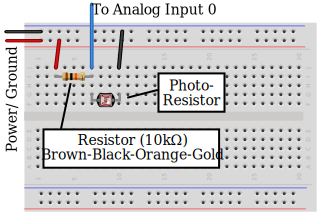
\includegraphics[width=\tw]{input-light-annotated.svg.pdf}
\end{minipage}
\hfill
\begin{minipage}[t]{0.49\tw}
  \vspace{0.1in}
  \begin{Verbatim}[gobble=3,fontsize=\small]
    int pin_light = A0;

    void setup() {
      Serial.begin(9600);
    }

    void loop() {
      int light_level = analogRead( pin_light );
      Serial.println( light_level );
      delay(1000);
    }
  \end{Verbatim}
\end{minipage}

